\documentclass[conference]{IEEEtran}


\usepackage[table]{xcolor}
\usepackage{cite}
\usepackage{url}
\usepackage[pdftex]{graphicx}
\usepackage{pifont}
\usepackage{tikz}
\usetikzlibrary{positioning}


\begin{document}


\title{Predicting Mutation Score Using Source Code\\and Test Suite Metrics}


\author{\IEEEauthorblockN{Kevin Jalbert, Jeremy S. Bradbury}
\IEEEauthorblockA{Software Quality Research Group\\
University of Ontario Institute of Technology\\
Oshawa, Ontario, Canada\\
\{kevin.jalbert, jeremy.bradbury\}@uoit.ca}}


\maketitle


\begin{abstract}
Traditionally mutation testing has been used to evaluate the effectiveness of test suites and provide confidence in the testing process. Mutation testing involves the creation of many versions of a program -- each with a single syntactic fault. A test suite is evaluated against these program versions (mutants) in order to determine the percentage of mutants a test suite is able to identify (mutation score). A major drawback of mutation testing is that even a small program may yield thousands of mutants and can potentially make the process cost prohibitive. To improve the performance and reduce the cost of mutation testing, we propose a machine learning approach to predict the mutation score based on source code and test suite metrics.
\end{abstract}


\IEEEpeerreviewmaketitle


\section{Introduction}
\label{sec:introduction}
Mutation testing traditionally has been used as a coverage technique to evaluate the effectiveness of test suites and provide confidence in the testing process~\cite{DLS78, OAL06, JH10}. For over 30 years, mutation has been applied to software written in programming languages including C~\cite{DM96, JH08}, Fortran~\cite{KO91}, Java~\cite{MKO02, BCD06} and more. Furthermore, mutation testing has also been applied to other non-programming artifacts such as formal specification languages~\cite{ABM98} and spreadsheets~\cite{AE09}.

Mutation testing uses a set of \emph{mutation operators} to generate faulty versions of a program called \emph{mutants}. Mutation operators are created based on an existing fault taxonomy and each operator usually corresponds to a specific type of fault. A mutant is identical to the original program except that it contains a single mutation -- ``\emph{a single syntactic change that is made to a program statement.}''~\cite{KO91}. A test suite is evaluated against a set of mutants to determine the \emph{mutation score}. The mutation score is defined as the percentage of non-equivalent mutants that are detected (\emph{killed}) by a test suite. The better a test suite, the more mutants will be killed and thus the higher the mutation score.

A major drawback of mutation testing is that even a small program may yield hundreds or thousands of mutants potentially making the process cost prohibitive in comparison to other coverage metrics such as statement or branch coverage. Several approaches have been proposed in the literature to improve mutation testing performance and scalability~\cite{OU00}:

\textbf{``Do fewer'' approach:} this category of optimizations aim to decrease the computational cost of mutation testing by reducing the number of mutants that a test suite is evaluated against. The most popular example from this category is selective mutation -- the use of a subset of mutation operators that have been empirically shown to be as effective as using an entire set of operators~\cite{OLR+96}. Another example of a ``do fewer'' approach is to randomly sample mutants~\cite{Won93}.

\textbf{``Do smarter'' approach:} this category of optimizations aim to decrease the cost of mutation testing by improving the actual mutation testing technique. For example, weak mutation \emph{``...is an approximation technique that compares the internal states of mutant and original program immediately after execution of the mutated portion of the code (instead of comparing the program output)''}~\cite{OU00}.

\textbf{``Do faster'' approach:} this category of optimizations aim to reduce the cost of mutation testing by focusing on performance. For example, one ``do faster'' approach improves compilation time using schema-based mutation -- \emph{``...encodes all mutations into one source level program...''}~\cite{OU00}.

As an alternative to the above techniques, we propose a ``do fewer and smarter'' technique for mutation testing at a unit level.  When mutation testing is used for the creation or improvement of a test suite,  the test suite will often have to be applied to the mutants in an iterative fashion as tests are added, removed and modified. Furthermore, the effects on the mutation score after each iteration have to be observed. We propose to replace at least some of these intermediate test suite evaluations on mutants with mutation score prediction and thus decrease the number of mutants that have to be evaluated using a test suite. Our proposed approach uses machine learning to predict the mutation score based on a combination of source code and test suite metrics of the code unit under test.

In the Section~\ref{sec:background} we describe the machine learning technique, the mutation testing tool and the metrics gathering tools used in our research. In Section~\ref{sec:approach} we describe our overall approach to mutant score prediction. We also discuss the integration of the tools described in the previous section, into our approach. In Section~\ref{sec:case_study} we apply our approach to an open source project and discuss the effectiveness of our prediction based on this preliminary evaluation. Finally, in Sections~\ref{sec:related_work}~\&~\ref{sec:conclusions_future_work} we discuss related work, conclusions, and future work.


\section{Background}
\label{sec:background}
In this section we describe the background techniques and tools used in our research. In particular, we discuss LIBSVM, support vector machine library, Javalanche, a mutation testing tool, the Eclipse Metrics Plugin, used for gathering source code metrics, and EMMA, used for acquiring test suite metrics. All tools were selected based on several criteria: (1) ability to execute command-line using a script, (2) ability to export output reports and (3) ability to fulfill the needs of our research.


\subsection{LIBSVM -- a library for support vector machines}
\label{subsec:libsvm}
A support vector machine (SVM) is an example of a linear discrimination machine learning technique and assumes that ``...\emph{instances of a class are linearly separable from instances of other classes}''~\cite{ALP04}. In other words, a SVM learns the linear discriminant of a set of data. SVMs are capable of learning how a set of features inform the classification of a data item. It can also be trained on known data items (in which the features and category are present), and then used to predict the category of  unknown data items (in which only the features are present).

Traditionally, SVMs have been used for two-group classification problems~\cite{CV95} but have also been generalized to \emph{n}-group classification problems. In a two-group classification problem this approach identifies an optimal separating hyperplane that divides the set of data into two groups based on a set of support vectors (i.e., features). In other words, the goal is to maximize the distance from the closest data points on both sides of the hyperplane to the hyperplane itself~\cite{ALP04}.

In our research we use LIBSVM (version 3.11), a SVM library capable of solving \emph{n}-group classification problems~\cite{CL11}. LIBSVM was chosen because it provides a command-line interface that could be easily integrated with the other tools used in our approach.


\subsection{Javalanche -- a mutation testing tool for Java}
\label{subsec:javalanche}
Mutation testing has previously been described in Section~\ref{sec:introduction}. In our research we use Javalanche (version 0.4), a mutation testing tool for Java~\cite{SZ09} that applies a subset of the method-level mutation operators to source code. Method-level operators are the most common set of mutation operators applied to procedural programming languages and each method-level mutation defines a syntactic change to an operator, operand or statement in a program. Javalanche uses a subset of the method-level mutation operators (replace constant, negate jump, arithmetic replace, remove call, replace variable, absolute value, unary operator) . These selected operators provide a close approximation of the effectiveness of using the entire set of method-level operators at a reduced cost~\cite{OLR+96}.

We chose Javalanche for our research because it is customizable and extensible, therefore allowing us to modify Javalanche to calculate unit mutation scores and output a richer set of results. We plan to further take advantage of Javalanche's extensibility in the future by adding object-oriented mutation operators. Other benefits of Javalanche include: full integration with JUnit and the use of mutation schemas to improve performance.

\subsection{Eclipse Metrics Plugin -- a source code metrics tool}
\label{subsec:Metrics}
Source code metrics measure knowledge of a project's source code through the use of code analysis. Source code metrics give insight into various aspects of the source code including it's complexity, size, coupling, cohesion as well as object-oriented attributes~\cite{SCE05,McCa76,Kan02,HWY09,Hend95,SRD12}.

In our research, we use the Eclipse Metrics Plugin (version 1.3.8.20100730-001) to acquire source code metrics of the methods and classes under test~\cite{Metrics}. We selected this tool as it provides a comprehensive set of metrics for Java programs.
We use Eclipse Metrics Plugin to collect metrics for feature sets \ding{172}, \ding{174} and \ding{175} from Table~\ref{tab:metrics}.

\begin{table}[!t]
  \centering
  \rowcolors{2}{gray!30}{gray!20}
  \begin{tabular}{|l|l|l|l|}
    \hline
    \rowcolor[RGB]{169,196,223}
    \textbf{Metrics} & \textbf{Description} & \textbf{Scope} & \textbf{Set} \\

    % Set 1: Source Code Metrics
    \hline MLOC & Method lines of code & Method & \ding{172} \\
    \hline NBD & Nested block depth & Method & \ding{172} \\
    \hline VG & McCabe cyclomatic complexity & Method & \ding{172} \\
    \hline PAR & Number of parameters & Method & \ding{172} \\
    \hline NORM & Number of overridden methods & Class & \ding{172} \\
    \hline NOF & Number of attributes & Class & \ding{172} \\
    \hline NSC & Number of children & Class & \ding{172} \\
    \hline DIT & Depth of inheritance tree & Class & \ding{172} \\
    \hline LCOM & Lack of cohesion of methods & Class & \ding{172} \\
    \hline NSM & Number of static methods & Class & \ding{172} \\
    \hline NOM & Number of methods & Class & \ding{172} \\
    \hline SIX & Specialization index & Class & \ding{172} \\
    \hline WMC & Weighted method per class & Class & \ding{172} \\
    \hline NSF & Number of static attributes & Class & \ding{172} \\

    % Set 2: Coverage Metrics
    \hline BCOV & Basic blocks covered in code unit & Class & \ding{173} \\
    \hline BTOT & Total basic blocks for code unit & Class & \ding{173} \\

    % Set 3: Accumulated Source Code Metrics
    \hline SMLOC & Sum of MLOC of methods & Class & \ding{174} \\
    \hline SNBD & Sum of NBD of methods & Class & \ding{174} \\
    \hline SVG & Sum of VG of methods & Class & \ding{174} \\
    \hline SPAR & Sum of PAR of methods & Class & \ding{174} \\
    \hline AMLOC & Average of MLOC of methods & Class & \ding{174} \\
    \hline ANBD & Average of NBD of methods & Class & \ding{174} \\
    \hline AVG & Average of VG of methods & Class & \ding{174} \\
    \hline APAR & Average of PAR of methods & Class & \ding{174} \\

    % Set 4: Accumulated Test Case Metrics
    \hline STMLOC & Sum of MLOC of test methods & Class/Method & \ding{175} \\
    \hline STNBD & Sum of NBD of test methods & Class/Method & \ding{175} \\
    \hline STVG & Sum of VG of test methods & Class/Method & \ding{175} \\
    \hline STPAR & Sum of PAR of test methods & Class/Method & \ding{175} \\
    \hline ATMLOC & Average of MLOC of test methods & Class/Method & \ding{175} \\
    \hline ATNBD & Average of NBD of test methods & Class/Method & \ding{175} \\
    \hline ATVG & Average of VG of test methods & Class/Method & \ding{175} \\
    \hline ATPAR & Average of PAR of test methods & Class/Method & \ding{175} \\

    % Set 5: Number of Tests
    \hline NOT & Number of tests &  Method & \ding{176} \\
    \hline SNOT & Sum of NOT of methods & Class & \ding{176} \\
    \hline ANOT & Average of NOT of methods & Class & \ding{176} \\
    \hline
  \end{tabular}
  \caption{The set of metrics used in our research. Each set of metrics correspond to a particular feature set (\ding{172}: Source Code Metrics, \ding{173}: Coverage Metrics, \ding{174}: Accumulated Source Code Metrics, \ding{175}: Accumulated Test Case Metrics, \ding{176}: Number of Tests Cases.)}
  \label{tab:metrics}
  \vspace{2mm}
  \hrule
\end{table}


\subsection{EMMA -- a test suite coverage tool}
\label{subsec:emma}
Test suite metrics can be gathered using similar technique to those used in the gathering of source code metrics. In fact, since we focus on JUnit test cases (which are Java classes) we can actually use the Eclipse Metrics Plugin to gather some of the test suite metrics. To gather other test suite metrics we use the tool EMMA (version 2.0.5312) which is capable of determining the statement and basic block coverage of a test suite~\cite{EMMA}. We use Emma to acquire metrics for feature set \ding{173} and \ding{176} from Table~\ref{tab:metrics}.


\section{Approach}
\label{sec:approach}
We now describe our approach to determining the mutation score of a unit under test based on source code and test suite metrics. In Section~\ref{subsec:training} we outline the process for collecting our initial data and training the SVM (see Figure~\ref{fig:process}) and in Section~\ref{subsec:prediction} we describe how to use the SVM for prediction and cross-validation.

\begin{figure}[!t]
  \centering
  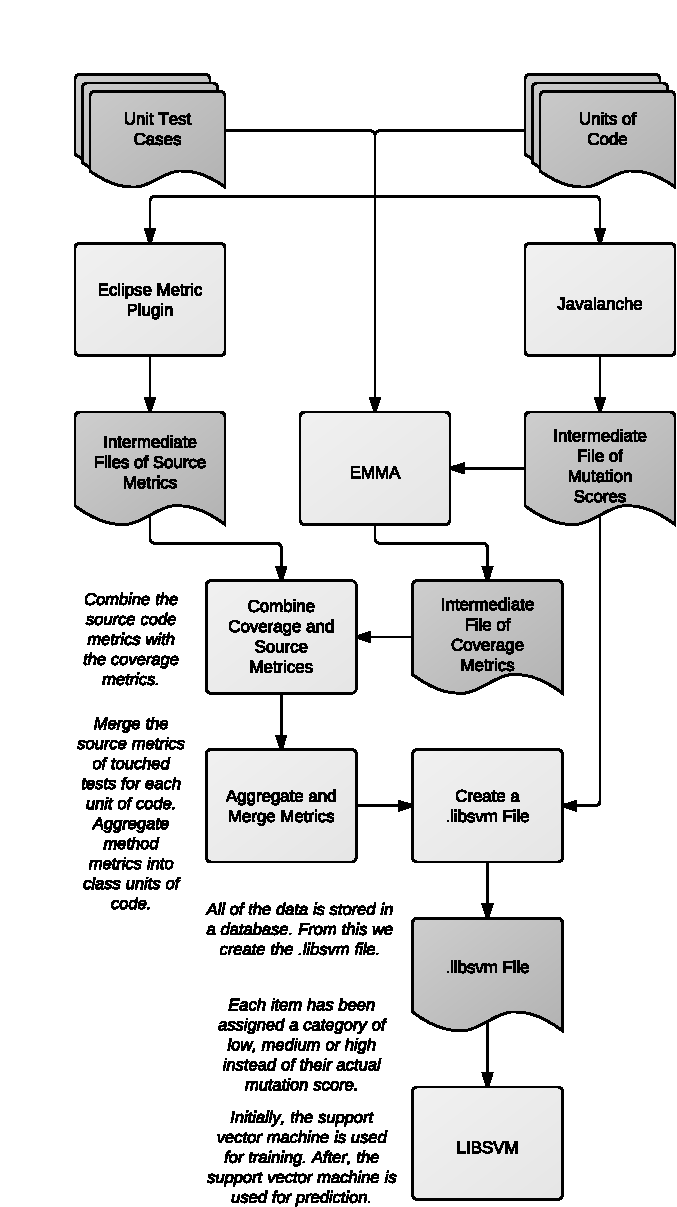
\includegraphics[width=7cm]{figures/process.pdf}
  \caption{Our training process -- using source code and test suite metrics to determine mutation score for a unit under test.}
  \label{fig:process}
  \vspace{2mm}
  \hrule
\end{figure}


\subsection{Training}
\label{subsec:training}
The input that our training process requires is a set of units of code in which each unit of code has a corresponding set of unit test cases. Both the units under test and test cases (i.e., JUnit tests) are Java source files.

The first step of our process is to collect the two types of data required to train the SVM:

\textbf{Category Data:} Javalanche is used to generate the mutants of all units in the project under test. In addition to mutant generation, Javalanche also performs the mutation testing by executing the required tests for each mutant, although it currently does not exclude equivalent mutants from the analysis. For our research, we added a new analyzer component to Javalanche that outputs an intermediate text file of mutation scores of the covered units (methods and classes). This intermediate text file also contains a list of every test that was executed for each method.

\textbf{Feature Data:} The feature data is comprised of the source code and test suite metrics. We use the tools described in Section~\ref{sec:background} to gather the metrics of the units of code under test and the unit test cases. The following will references the metric sets from in Table~\ref{tab:metrics}. We gather metric set \ding{172} using the Eclipse Metric Plugin and we also accumulate the test code units metrics to form metric set \ding{175}. EMMA is used to collect metric set \ding{173} and \ding{176} by determining the coverage of each method by only examining the set of executed tests for each method-level code unit. All the tools produce intermediate files of data, which we combine together into a database. As classes are composed of one-to-many methods, we aggregate and merge metrics from the contained methods to generate the set of accumulated class metrics (see set \ding{174} in Table~\ref{tab:metrics}).

Next, we create a .libsvm file containing the category and feature data from the database. Instead of predicting a specific mutation score percentage, we categorize all mutation scores as \textit{low, medium, high} which reduces the mutation score prediction to a three-group classification problem. The ranges are determined based on the distribution of the mutation scores in our training data (further explained in Section~\ref{subsec:results}). Finally, the .libsvm file is passed into LIBSVM to complete the training process.


\subsection{Prediction}
\label{subsec:prediction}
Once we have trained the SVM, we can then use the SVM for prediction. We can predict the category of an unknown unit of code by first extracting the source code and test suite metrics. The extracted features are then passed into the SVM which will then be assigned a category of \textit{low, medium, high} for the mutation score.  Currently, our approach only predicts mutation scores within a project. That is, the training and prediction data both come from the same project repository.


\section{Case Study: JGAP}
\label{sec:case_study}
A preliminary evaluation of our mutation score predictor was preformed on JGAP (version 3.6.1), an open source genetic algorithm and genetic programming framework for Java, which was selected due to its comprehensive JUnit test suite~\cite{JGAP}. We decided to use an open source project that is large enough to contain many mutants, as well as a mature test suite. Basic source code metrics for JGAP are provided in Table~\ref{tab:jgap_source_stats}. JGAP contains 1387\footnote{JGAP has 1412 JUnit test cases in total, however 25 of the tests caused errors in the Javalanche tool and were removed.} usable JUnit test cases. For JGAP Javalanche generated 32031 mutants using the method-level mutation operators (see Section~\ref{subsec:javalanche}) of which only 18378 were actually covered by JGAP's test suite. We only considered the set of covered mutations in our approach as the mutations not covered contained no associated test cases. Considering only the covered mutants, JGAP's test suite killed 13698 mutants in 688 minutes and 43 seconds\footnote{Ran on Intel Core i7-870 processor @ 2.93 GHz, with no parallel task execution in Javalanche} resulting in an overall mutation score of 74.53\%.

\begin{table}[!t]
  \centering
  \rowcolors{2}{gray!30}{gray!20}
  \begin{tabular}{|l|r|r|}
    \hline
    \rowcolor[RGB]{169,196,223}
    \textbf{JGAP Source Artifacts} & \textbf{\# in Source} & \textbf{\# in Test} \\
    \hline Classes & 415 & 180 \\
    \hline Methods & 3017 & 1626 \\
    \hline LOC & 28975 & 19556 \\
    \hline JUnit Test Cases & -- & 1412\footnotemark[1] \\
    \hline
  \end{tabular}
  \caption{The amount of classes, methods, lines of code (LOC), and JUnit test cases in the JGAP repository}
  \label{tab:jgap_source_stats}
  \vspace{2mm}
  \hrule
\end{table}


\subsection{Results}
\label{subsec:results}
We gathered 695 method-level data points and 127 class-level data points from JGAP. We first decided to view the distribution of JGAP's mutation scores, which are shown in Figure~\ref{fig:mutation_distributions}. It is clearly obvious that the distribution for both classes and methods are more heavily dense for high mutation scores.

\begin{figure*}[!t]
  \centering
  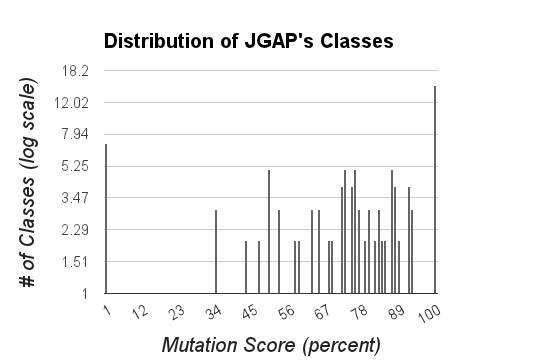
\includegraphics[width=8cm]{figures/class_distribution.png}
  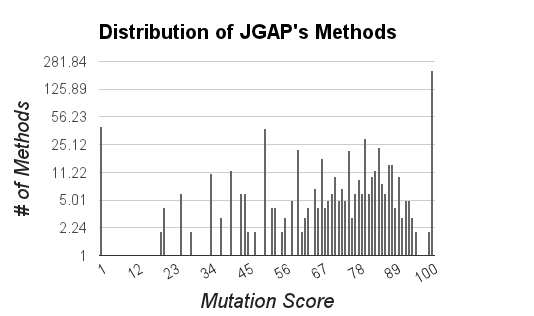
\includegraphics[width=8cm]{figures/method_distribution.png}
  \caption{The mutation score distribution (in log scale) of JGAP's classes and methods that can be used for training.}
  \label{fig:mutation_distributions}
  \vspace{2mm}
  \hrule
\end{figure*}

As mentioned in Section~\ref{subsec:training} we categorize the collected data into three groups of \textit{low, medium, high} based on their mutation scores. Ideally we would like to have sufficient data coverage for the complete range of mutation scores, such that we can train the SVM using simple categories such as 0\%--33\% (\textit{low}), 33\%-66\% (\textit{medium)} and 66\%-100\% (\textit{high}). Given our situation of not being able to split up the collected data easily across the mutation scores we instead decided to categorize our data such that one third of our data will fall into each category. This results in varying mutation score ranges for each category for class- and method-level data as shown in Table~\ref{tab:results_details}.

\begin{table}[!t]
  \centering
  \rowcolors{2}{gray!30}{gray!20}
  \begin{tabular}{|l|r|r|}
    \hline
    \rowcolor[RGB]{169,196,223}
    \textbf{Category} & \textbf{Class Mutation Score} & \textbf{Method Mutation Score} \\
    \hline low & 0.00\% -- 62.75\% & 0.00\% -- 66.66\% \\
    \hline medium & 62.75\% -- 83.25\% & 66.66\% -- 90.90\% \\
    \hline high & 83.25\% -- 100.00\% & 90.90\% -- 100.00\% \\
    \hline
  \end{tabular}
  \caption{The mutation score ranges that equally partition the datasets into three categories.}
  \label{tab:results_details}
  \vspace{2mm}
  \hrule
\end{table}

\begin{figure}[!h]
  \scriptsize
  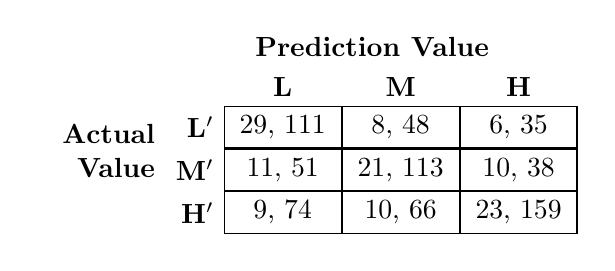
\begin{tikzpicture}[
  box/.style={draw,rectangle,minimum size=0.5cm,text width=1.25cm,align=center}]
    \matrix (confusion_matrix) {
      \node (actual_low_prediction_low)
      [box,
        label=left:\(\mathbf{L'}\),
        label=above:\(\mathbf{L}\)
      ] {29, 111};
      &
      \node (actual_low_prediction_medium)
      [box,
        label=above:\(\mathbf{M}\)
      ] {8, 48};
      &
      \node (actual_low_prediction_medium)
      [box,
        label=above:\(\mathbf{H}\)
      ] {6, 35};
      \\
      \node (actual_medium_prediction_low)
      [box,
        label=left:\(\mathbf{M'}\)
      ] {11, 51};
      &
      \node (actual_medium_prediction_medium)
      [box] {21, 113};
      &
      \node (actual_medium_prediction_high)
      [box] {10, 38};
      \\
      \node (actual_high_prediction_low)
      [box,
        label=left:\(\mathbf{H'}\)
      ] {9, 74};
      &
      \node (actual_high_prediction_medium)
      [box] {10, 66};
      &
      \node (actual_high_prediction_high)
      [box] {23, 159};
      \\
    };
    \node [left=-.1cm of confusion_matrix,text width=1.5cm,align=right] {\textbf{Actual \\ Value}};
    \node [above=-.1cm of confusion_matrix] {\textbf{Prediction Value}};
  \end{tikzpicture}
  \caption{Confusion matrix for (class, method) mutation score prediction on JGAP using all feature sets from Table~\ref{tab:metrics}. The first value in each cell represents the class value while the second represents the method value. \(\mathbf{L}\) = Low, \(\mathbf{M}\) = Medium and \(\mathbf{H}\) = High.}
  \label{fig:confusion_matrix}
  \vspace{2mm}
  \hrule
\end{figure}

To evaluate our results we decided to perform a 10-fold cross-validation of our datasets due to the small amount of data acquired from this experiment. Effectively, this splits up our dataset into \emph{10} equal-sized partitions and the SVM internally train on $\emph{9}$ sets and predict the last. This process is repeated \emph{10} times where a different partition is selected for prediction each time. Finally all the individual prediction accuracies are tallied and averaged for a cross-validation accuracy of \emph{10}-folds. Our achieved cross-validation accuracy of JGAP (with all features from Table~\ref{tab:metrics}) was 57.48\% for class mutation scores and 55.11\% for method mutation scores. Figure~\ref{fig:confusion_matrix} illustrates the confusion matrix of the predicted values made by the SVM for our three categories. It is also worth mentioning that our achieved accuracy outperforms random (which has an accuracy of 33.33\% given our category distributions) by 24.15\% for classes and 21.78\% for methods. We re-conducted the cross-validation using subsets of our feature set and found that the combination of features slightly improves the prediction accuracy (see Table~\ref{tab:subset_accuracy}). A further analysis of the acquired metrics used as the feature set in LIBSVM would prove useful in understanding the relevant and important metrics in mutation score prediction.

\begin{table}[!t]
  \centering
  \rowcolors{2}{gray!30}{gray!20}
  \begin{tabular}{|l|r|r|}
    \hline
    \rowcolor[RGB]{169,196,223}
    \textbf{Set} & \textbf{Class Accuracy} & \textbf{Method Accuracy} \\
    \hline \ding{172} & 53.54\% & 48.77\% \\
    \hline \ding{173} & 49.61\% & 47.63\% \\
    \hline \ding{174} & 45.67\% & 49.78\% \\
    \hline \ding{175} & 54.33\% & 33.96\% \\
    \hline \ding{176} & 44.88\% & 45.47\% \\
    \hline
  \end{tabular}
  \caption{The cross validation (10-folds) accuracy of each feature subset of all the features. The sets reference the features from Table~\ref{tab:metrics}.}
  \label{tab:subset_accuracy}
  \vspace{2mm}
  \hrule
\end{table}


\section{Related Work}
\label{sec:related_work}
The use of software metrics to locate faults in source code has been well researched. For example, Koru et al. utilized static software measure along with defect data at the class level to predict bugs using machine learning~\cite{KL05}. Similarly, Gyimothy et al. used object-oriented metrics with logistic regression and machine learning techniques to identify faulty classes in open source software~\cite{GFS05}. Finally, design level metrics were used with a linear prediction model to determine the estimated maintainability and error prone modules of large software systems~\cite{MKPS00}. Our work is unique in comparison to these previous works since we not only use source code metrics but we also use test suite metrics to enhance our predication capabilities.


\section{Conclusions \& Future Work}
\label{sec:conclusions_future_work}
Our technique for predicting mutation score using source code and test suite metrics achieved an accuracy of 57.48\% and 55.11\% for classes and methods respectively -- outperforming random. These results have not been optimized and we believe that with further enhancements and a more tailored feature set we may be able to increase our prediction accuracy.

Our approach currently only used a subset of the traditional mutation operators. Obviously there are some limitations of this, we are missing a whole class of mutation operators that operator on object-oriented aspects of the system under test. We plan to address this issue in future work by extending Javalanche to include more mutation operators.

Currently we have applied our predictive technique to a single open source project -- JGAP. Additionally, we performed training and prediction from the same project. As stated by Kitchenham and Mendes \textit{``It is invalid to select one or two datasets to `prove' the validity of a new technique because we cannot be sure that, of the many published datasets, those chosen are the only ones that favour the new technique''}~\cite{KM09}. Thus, we plan to evaluate more open source projects using our prediction technique to better assess the prediction accuracy. With more data we plan to investigate whether cross-project models are valid for mutation score prediction. We would like to consider projects with more mutation scores to explore the variation in prediction accuracy between strong and weak test suites. Finally by considering more projects we can also explore the validity of the proposed technique.


\bibliographystyle{IEEEtran}
\bibliography{references}


\end{document}
